\chapter{Bevezetés}
\label{chapIntroduction}
\paragraph{}
A szoftverfejlesztés a mai világunk egyik alapköve. 
Az informatika világa és a mi hétköznapi eszközeink sem lennének képesek fejlődni a szorgos programozók munkája nélkül. 
Azonban a szoftver fejlesztés nem egy egyszerű dolog, főleg ha egy komplex programozási feladatra van szükség. 
Ilyenkor szinte biztosan nem egy ember fogja elkészíteni ezeket a programokat, így a munka kódolás része kevesebb feladatot ró a fejlesztőre viszont számos egyéb feladattal kell szembe néznie.

\paragraph{}
Ezek a feladatok (ha jól elő vannak készítve) nagyon könnyen vehető akadályok. 
Ha minden új munkatársnak bemutatják hogy milyen struktúrában kell kódolnia vagy vannak egyéb eszközök segítik a munkáját.
Ezek lehetnek verziókövetőrendszerek, automatikus tesztelési környezet vagy akár csak a dokumentum legenerálásában segítő alkalmazás.

A programozókra komoly munka és rengeteg egyeztetés várna, ha nem léteznének úgynevezett verzió követő rendszerek.
Nem is lehetne olyan szoftver gyártó céget mondani mely nem használná valamely formában a Git-et.

Persze ezen felül ha többen dolgoznak egy kódon akkor a csapatmunka gördülékenységét segíti elő bizonyos szabályok lefektetése.
Az ugyan olyan formátumú kód használata elengedhetetlen komplex programok megírásakor.
Vagy a dokumentáció is, hogy a kód később is vagy egy új kolléga számára is egyértelmű legyen.

A Continuous Integration – azaz a folyamatos integráció
---HALO---

A csapatban való munka legalább olyan fontos részét alkotja a modern szoftverfejlesztésnek mint a munkálatokat segítő rendszerek.
Ha egy mai informatikai céget meglátogatunk, azt láthatjuk hogy a programozók nem elszeparáltan hanem egy közös térben dolgoznak.
Például egyre népszerűbb a scrum módszer bevezetése az irodákban és minden reggel ennek megfelelően egy közös megbeszéléssel kezdőik.

A csapatmunkát komoly támogatási háttérrel szükséges ellátni. 
Gondok itt arra, hogy lehetőséget kell adni minden fejlesztő számára, hogy a fejlesztés állapotát nyomon tudják követni és a mások munkáját is könnyen feltudják használni vagy esetenként módosítani tudják azt. 
Ezeket a lehetőségeket nem egy egyszerű feladat megteremteni legyen szó tíz vagy akár százfős irodáról.

\paragraph{}
Ez a téma az informatika nem annyira szembetűnő oldaláról mutatja be. 
A mai világban gyakran hajlamosak vagyunk megfeledkezni arról, hogy az a kép amit elkattintunk a telefonunkkal hogyan is kerül fel a felhőbe és onnan a asztali számítógépünkre vagy akár a barátainkhoz valamilyen közösségi média platform használatának segítségével.
Nem egy program megszületését dokumentáltam hanem sokkal inkább azt, hogy egy komplex programhoz milyen háttér eszközök kellenek hogy elkészüljön.
\pagebreak
\section{Motiváció}
\label{chapMotivation}

\paragraph{}
Mostanra az informatikusnak tanulók között is sokkal izgalmasabb egy mobilfejlesztés vagy egy webfejlesztés.
Az látszik, az van előtérben, végül is az ő munkájuk ami igazán eljut a végfelhasználókhoz.
Ez teljesen megérthető hiszen a színes izgő-mozgó képek tengerével hogyan is vehetné fel a versenyt egy még a Mátrix c. kultuszfilmben is csak keveset látott terminál ablak fekete-zöld karakteri.
Pedig ez a világ az ami lehetővé teszi az eszközök közötti összeköttetést és a csillogó képekkel teli megjelenést.
Az ember azt gondolná hogy a programozók pontosan ismerik ezt a világot, pedig vannak akik ennél is mélyebbre mennek.
Ezek az emberek a rendszerüzemeltetők és az ők titkolt és rejtett világuk.
Pontosan ez tetszett meg nekem és ezért is szeretnék hasonló témában elkészíteni a feladatom.
Természetesen ez talán még nem elég ahhoz hogy egy ilyen témába mélyen beleássa  magát az ember.
Már régebben is az foglalkoztatott hogy bizonyos játékoknak hogyan tudnék saját szervert csinálni hogy a barátainkkal igazán szabadon élvezhessük a játékok adta élményeket.

\paragraph{}
A Miskolci Egyetem Mérnökinformatikai szakán eltöltött éveim során próbáltam a lehető legtöbb olyan sávot választani a tantervi hálóból ami nem fejlesztéssel hanem üzemeltetéssel foglalkozik. 
A fejlesztés sem egy teljesen unalmas ága az informatikának, viszont számomra az üzemeltetés egy sokkal változatosabb világba varázsol el.
A jövő is nagy számítási teljesítmények (Big Data, Deep Learning) felé mutat amelyet nem titkolt célom még a technológia hajnalán elsajátítani. 
Úgy gondolom, hogy a mai fejlesztési feladatinak még nagyobb szüksége van a stabíl, jól működő és állandóan rendelkezésre álló supportra. 
Ezért is ragadtam meg a lehetőséget mikor Dr. Tóth Zsolt konzulensem felajánlott egy projekt munkát a Miskolci Egyetem Informatika Intézetében. 

\paragraph{}
Ez a projekt az ILONA beltéri helymeghatározó rendszernek a fejlesztése során szükségessé vált automatizált tesztelési rendszer és környezet kialakítása volt. 
Mikor elkezdtem foglalkozni a témával még jobban megtetszett az üzemeltetés és a support világa és ekkor gondoltam úgy, hogy ebből szakdolgozatot fogok írni. 
Ezzel a dolgozattal is rengeteg újat dolgot tanultam amit az egyetemi tanórák keretein belül soha sem tanultam volna meg. 

Számomra ez a projekt teljes mértékig szabad kezet adott.
A saját képzeletemnek és ismereteimnek megfelelően tudtam egy teljesen új rendszert megépíteni és mások számára elérhetővé tenni.
Időközben elkezdtem dolgozni is az egyetem mellett ahol ugyan így üzemeltetéssel tudok foglalkozni.
Sok ötletel tudtam eltanulni kollégáimtól és úgy gondolom én is tudtam nekik újat mutatni melyeket itt az egyetemen ezzel a projekttel tanultam meg.


Számomra nagyon fontos volt hogy egy olyan témával tudjak foglalkozni ami maradandó nyomot hagy az egyetemen.
Egy ilyen rendszert felépíteni és üzemeltetni jó lehetőség erre, hiszen a folyamatosan cserélődő fejlesztői csapat sokáig tudja majd használni.
A rendszer úgy van megtervezve hogy bővíthető legyen és esetleges extra igényeket is kitudjon szolgálni a IIT-s csapat számára.

\pagebreak
\section{Célkitűzés}
\label{chapGoal}
\paragraph{}
A célom azt volt, hogy a Miskolci Egyetem Általános Informatika Tanszékén az ILONA rendszeren dolgozó fejlesztőknek a munkáját segítsem. 
A fejlesztők jelenleg az építést és a tesztelést is manuálisan valósítják meg, ahogy ez a \ref{fig:jelenallapot} ábrán is látható. Ez a feladatom kiinduló állapota. 

\begin{figure}[h]
	\centering
	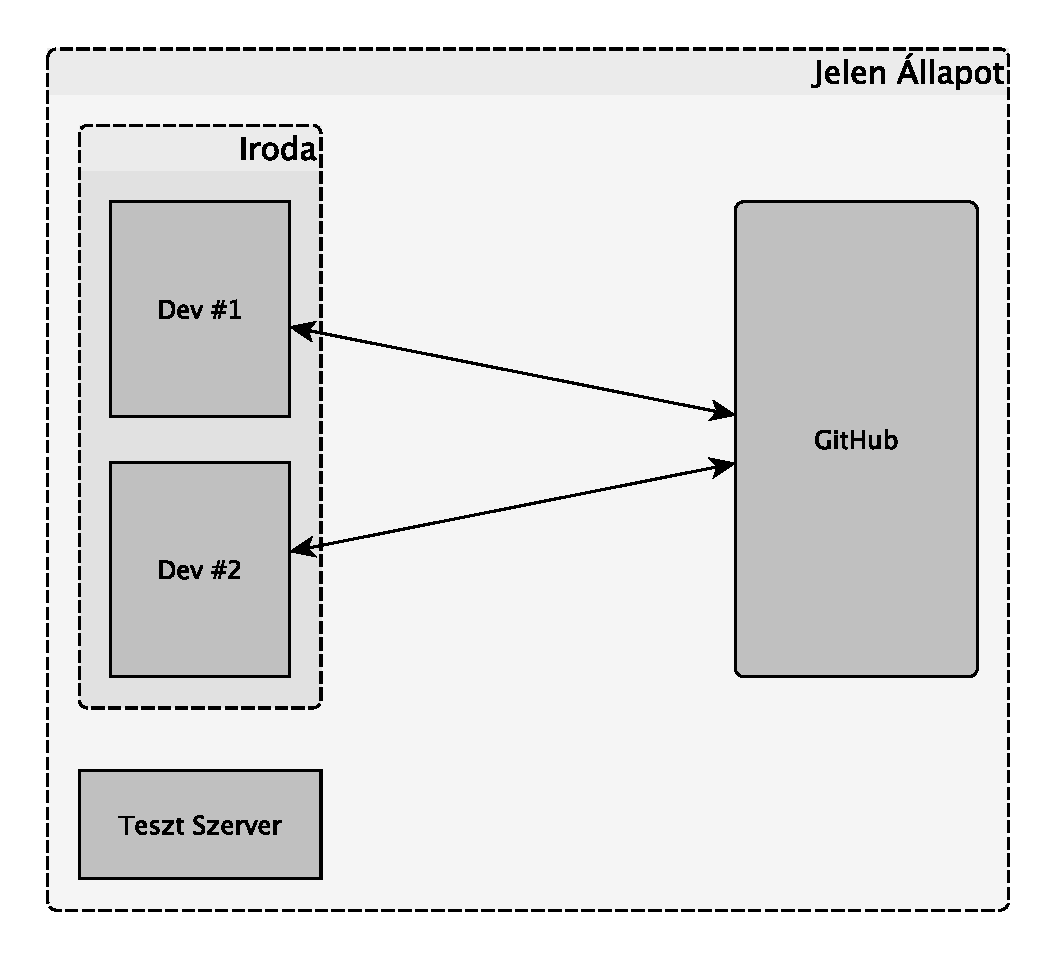
\includegraphics[width=0.7\linewidth]{figures/jelenallapot}
	\caption{Jelen Állapot}
	\label{fig:jelenallapot}
\end{figure}

Az új rendszernek a jelenlegi állapotnak több sajátosságát meg szerettem volna tartani és ezeken felül a már meglévő szerverekkel megvalósítani a rendszer működését. 
Fontosnak tartottam hogy a fejlesztők kizárólag a feladataik csökkenésével szembesüljenek és ne keljen új programokat, folyamatokat megtanulniuk. 
Kvázi ne látszódjon a háttérbe folyó változás és a jelenlegi rendszer szolgáltatás kiesésével se járjon az új rendszer bevezetése. 
Mivel az ILONA fejlesztése teljesen önerőből, támogatás nélkül valósul meg, ezért törekedtem arra hogy csak ingyenes, "opensource" alkalmazásokat használjak a feladathoz. 
Sikerült is ennek eleget tenni, minden komponens opensource és ingyenesen elérhető bárki számára az interneten.

A jelenlegi rendszer alapja az egyik legnépszerűbb ingyenes internetes verziókövető rendszer a GitHub. 
A GitHub-ot feltétlen meg akartam tartani az új rendszerben mivel egy elterjedten használt és kedvelt környezetnek tartom és ami még mellette szól az az ingyenessége. 
Természetesen lehetett volna saját git-et is használni viszont az egyetemi projekteken nem mindig csak a campuson dolgozunk és nem is kell mindig titokban tartani.

A mostani teszt szerver Maven segítségével építi és teszteli a megírt kódokat, ezért a következő amit a meglévő rendszerből át akartam vinni az újba az a Maven. 
A jelenlegi rendszer nem hatékony a munkavégzés során, mivel számos munkaidőt emészt fel a folyamat amely nem a fejlesztéssel kapcsolatos. 

\pagebreak
\paragraph{}
A fejlesztőknek az új rendszerben lényegében csak a GitHubbal és a kész JAR fájlokat tartalmazó repository szerverrel kell dolgozniuk a többi folyamatot automatikusan látná el a rendszer. 
A cél tehát egy olyan Automatikus Tesztelési Környezet megvalósítása, amely képes a GitHubról letölteni a kódokat akkor ha a kódban változás történik. 
Ezen felűl ha a tesztek és a buildelési folyamat is sikeresen végbement az elkészült fájlokat könnyen és szervezetten elérhetővé tennie egy repository szerveren. 
Ez a tervezett folyamat látható a \ref{fig:jovoallapot} ábrán. 


\begin{figure}[h]
	\centering
	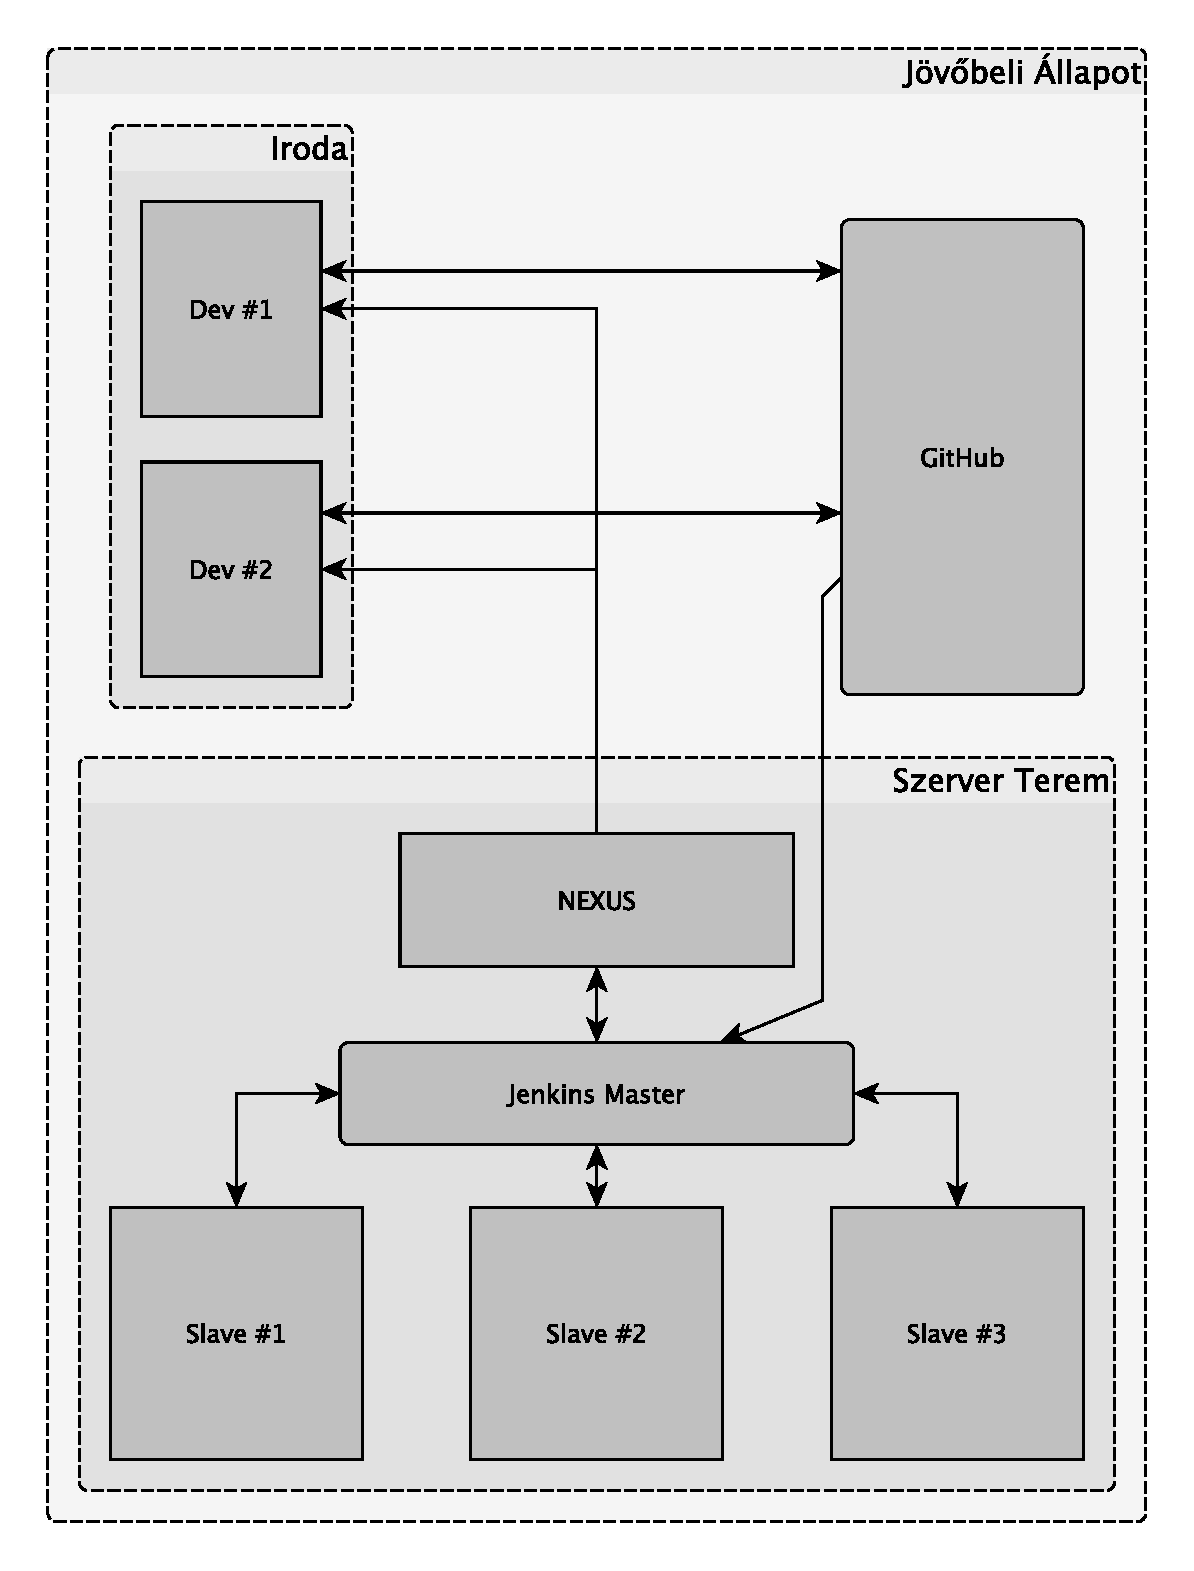
\includegraphics[width=0.7\linewidth]{figures/jovoallapot}
	\caption{Jövő Állapot}
	\label{fig:jovoallapot}
\end{figure}
